% !TEX program = XeLaTeX
% !TEX encoding = UTF-8
\documentclass[UTF8,nofonts]{article}
%{ctexart}


%\setCJKmainfont[BoldFont=FandolSong-Bold.otf,ItalicFont=FandolKai-Regular.otf]{FandolSong-Regular.otf}
%\setCJKsansfont[BoldFont=FandolHei-Bold.otf]{FandolHei-Regular.otf}
%\setCJKmonofont{FandolFang-Regular.otf}

\usepackage{url}
\usepackage{cancel}
\usepackage{xspace}
\usepackage{graphicx}
\usepackage{multicol}
\usepackage{multirow}
\usepackage{subfig}
\usepackage{amsmath}
\usepackage{amssymb}
%\usepackage[a4paper, width=180mm, top=18mm, bottom=22mm, includeheadfoot]{geometry}
\usepackage[a4paper, width=140mm, top=18mm, bottom=22mm, includeheadfoot]{geometry}
\usepackage{booktabs}
\usepackage{array}
\usepackage{verbatim}
\usepackage{caption}
%\usepackage{natbib}
\usepackage{booktabs}
\usepackage{float}
\usepackage{pdflscape}
\usepackage{mathtools}
\usepackage[usenames, dvipsnames]{xcolor}
\usepackage{afterpage}
\usepackage{pgf}
\usepackage{tikz}
\usepackage{dirtree}
\usepackage{amsfonts}
\usepackage{tkz-graph}


\newtheorem{definition}{Definition}[section]
\newtheorem{theorem}{Theorem}[section]
\newtheorem{lemma}{Lemma}
\newtheorem{proof}{Proof} [section]



\usepackage[toc, page, title, titletoc, header]{appendix}
\usepackage{marginnote}
\usepackage{tablefootnote}

%\renewcommand\appendixname{附\ 录}
%\renewcommand\appendixpagename{附\ 录}
%\renewcommand\appendixtocname{附\ 录}
\renewcommand\abstractname{Abstract}


\usepackage{perpage} %the perpage package
\MakePerPage{footnote} %the perpage package command

\usetikzlibrary{shapes.geometric}%
\usepackage{color}
%\usepackage[pages=some, placement=top]{background}
\usepackage{eso-pic}

\title{Multilateral Token Trade Protocol (MTTP)\\v0.6}
\author{
  daniel@mttp.io\\
  jay@mttp.io\\
  alex@mttp.io\\ 
  \\
  \textit{MTTP Foundation}\\
  \textit{http://mttp.io}\\
  \textit{foundation@mttp.io}\\
 }

\makeatletter
\def\CTEX@section@format{\Large\bfseries}
\makeatother

\makeatletter
\newenvironment{tablehere}
 {\def\@captype{table}}
 {}

\newenvironment{figurehere}
 {\def\@captype{figure}}
 {}
\makeatother

\newcommand\BackgroundPic{%
\put(0, 0){%
\parbox[b][\paperheight]{\paperwidth}{%
\vfill
\centering

\includegraphics[width=\paperwidth, height=\paperheight, %
%keepaspectratio]{images/background.jpg}%
]{images/background.jpg}%
\vfill
}}}


\begin{document}
\AddToShipoutPicture{\BackgroundPic}
\maketitle
This document is for informational purposes only and does not constitute an offer or solicitation to sell shares or securities. Any such offer or solicitation will be made only by means of a confidential offering memorandum and in accordance with the terms of all applicable securities and other laws.



\begin{abstract}
Multi-lateral token exchange protocol(MTTP) is an open protocol for decentralized exchange on the Ethereum blokchcian. MTTP is intended to serve as an open standard and common building block,  driving interoperability among decentralised applications(dAPPs) that incorporate exchange functionality.Trades are executed by a system of Ethereum smart contracts that are publicly accessible,  free to use, and that any dApp can hook into for taken exchanging.
\end{abstract}

\newpage

\tableofcontents
\newpage

\section{Background\label{sec: background}}

Blockchain\cite{staff2016blockchains}\cite{swan2015blockchain} technology was created to facilitate the cryptocurrency Bitcoin\cite{nakamoto2008bitcoin}. It is originally a decentralized system to enforce the financial agreements\cite{lamport1982byzantine}\cite{christidis2016blockchains}. The technology that underlies them could spread into other transactions: trading stock,  IP, buying and selling real estate, purchasing music and much more. Despite both consortium blockchain and private blockchain have been developed and implemented in few years, however the value only exists among the closed set of entities or internal entity. While fully public blockchain operates by having a large number of participants,  resulting in trust by numbers. According to coinmarketcap.com stats,  the total cryptocurrency market cap value has reached to 79 billions USD,  including 17 billions USD from Ethereum\cite{wood2014ethereum}.

Blockchain has massive influnce on the many areas,  particular in finance area. It is strongly believed that tokenization\cite{liu2016medical}\cite{christidis2016blockchains}\cite{swan2015blockchain} is a new solution. Asset tokenization can reduce the cost,  globalize the asset and increase the liquidation. We will see more dApps that require the use of these different tokens. As a result,  an open standard for exchange is critical to supporting this open economy.

A traditional exchange platform is based on peer-to-peer IOUs and blockchain technology. Firstly,  users need to deposit thier money or tokens into exchange’s wallet or bank account,  the their account will be credited some IOU. Thus,  users actually are trading the IOU in the exchange. Users have to file a ticket when they want to withdraw or sell the tokens.
In February 2014,  World largest bitcoin exchange “Mt. Gox” suspended trading,  closed its website and exchange service,  and filed for bankruptcy protection from creditors\cite{mcmillan2014inside}. Mt. Gox announced that approximately 850, 000 bitcoins belonging to customers and the company were missing and likely stolen,  an amount valued at more than \$ $450$ million at the time. Research showed less than 1% (7000 btc) of missing funds lost to attacks. In 2016,  Bitfinex was the subject of the Bitfinex hack. In it,  $72 million in bitcoin was stolen from the company's customer's accounts. Therefore,  lack of regulation is hurting bitcoin in many regions. It also aproves that the centralized exchange platform has those unavoidable risk.
We describe a protocol that facilitates decentralized exchange machanism of ERC20 tokens on the Ethereum blockchain to slove above issues. One of the strength for decentralization is not holding by any party,  thus stolen becomes impossible, which can build up the trust bewteen customers and exchange at a very low cost. In addition, this machanism has no time and region limits, but highly transparent and traceable features. All those features make trasaction more liquidatable and minimize the price difference.

\section{Market and Industry\label{sec: existingworks}}

There are some decentralized exchanges on blockchain technolegy like Ripple,  BitShares,  Openledger in open sourced community.
Ripple\cite{schwartz2014ripple} is a real-time gross settlement system,  currency exchange and remittance network operated by Ripple. Also called the Ripple Transaction Protocol (RTXP) or Ripple protocol,  it is built upon a distributed open source Internet protocol,  consensus ledger. Ripple’s solution is built around an open,  neutral protocol (Interledger Protocol or ILP\cite{thomas2015protocol}) to power payments across different ledgers and networks globally. It offers a cryptographically secure end-to-end payment flow with transaction immutability and information redundancy. Architected to fit within a bank’s existing infrastructure,  Ripple is designed to comply with risk,  privacy and compliance requirements.
BitShares\cite{schuhbitshares}\cite{schuh2015bitshares} is an industrial-grade financial blockchain smart contracts platform. The BitShares decentralized exchange - also known as “The DEX” is a next-generation cryptocurrency trading platform. The DEX is inherently decentralized,  enabling you to trade the BitShares core token (BTS) and a range of trustless price-stable,  market-pegged assets such as bitUSD,  bitCNY,  bitBTC,  bitGold and more. These assets can all be traded with zero counter-party risk,  putting you in total control of your funds. However,  Bitshares project has many limitations on itself.
The OpenLedger Dex\cite{openledger} is a cryptocurrency exchange. It allows users to exchange bitcoin into SmartCoins and then withdraw the smartcoins and convert them into cash through PayPal,  Ripple or NanoCard. Additionally,  openledger highly relys on BitShares 2.0 platform and Graphene Toolkit’s operation.
The Bancor\cite{bancor}\cite{hanson2012logarithmic} protocol enables built-in price discovery and a liquidity mechanism for tokens on smart contract blockchains. These “smart tokens” hold one or more other tokens in reserve and enable any party to instantly purchase or liquidate the smart token in exchange for any of its reserve tokens,  directly through the smart token’s contract,  at a continuously calculated price, according to a formula which balances buy and sell volumes.
“0x”\cite{warren20170x} is a protocol that facilitates low friction peer-to-peer exchange of ERC20\cite{ERC20} tokens on the Ethereum blockchain. The protocol is intended to serve as an open standard and common building block,  driving interoperability among decentralized applications (dApps) that incorporate exchange functionality. Trades are executed by a system of Ethereum smart contracts that are publicly accessible,  free to use and that any dApp can hook into. DApps built on top of the protocol can access public liquidity pools or create their own liquidity pool and charge transaction fees on the resulting volume. While,  0x protocol has many limitations including,  only accept simple OTC order; unclear competing mechanism among each exchanges; lack of protection mechanism for miners.
Due to above reasons and limitation,  centralized exchange is now still playing an important role in cryptocurrency market. Nevertheless,  Our team has inspired by both 0x protocol and payment channel and brought up a new solution for decentralized exchange protocol.


\section{Design Protocol\label{sec: protocol}}

\begin{center}
\begin{figurehere}
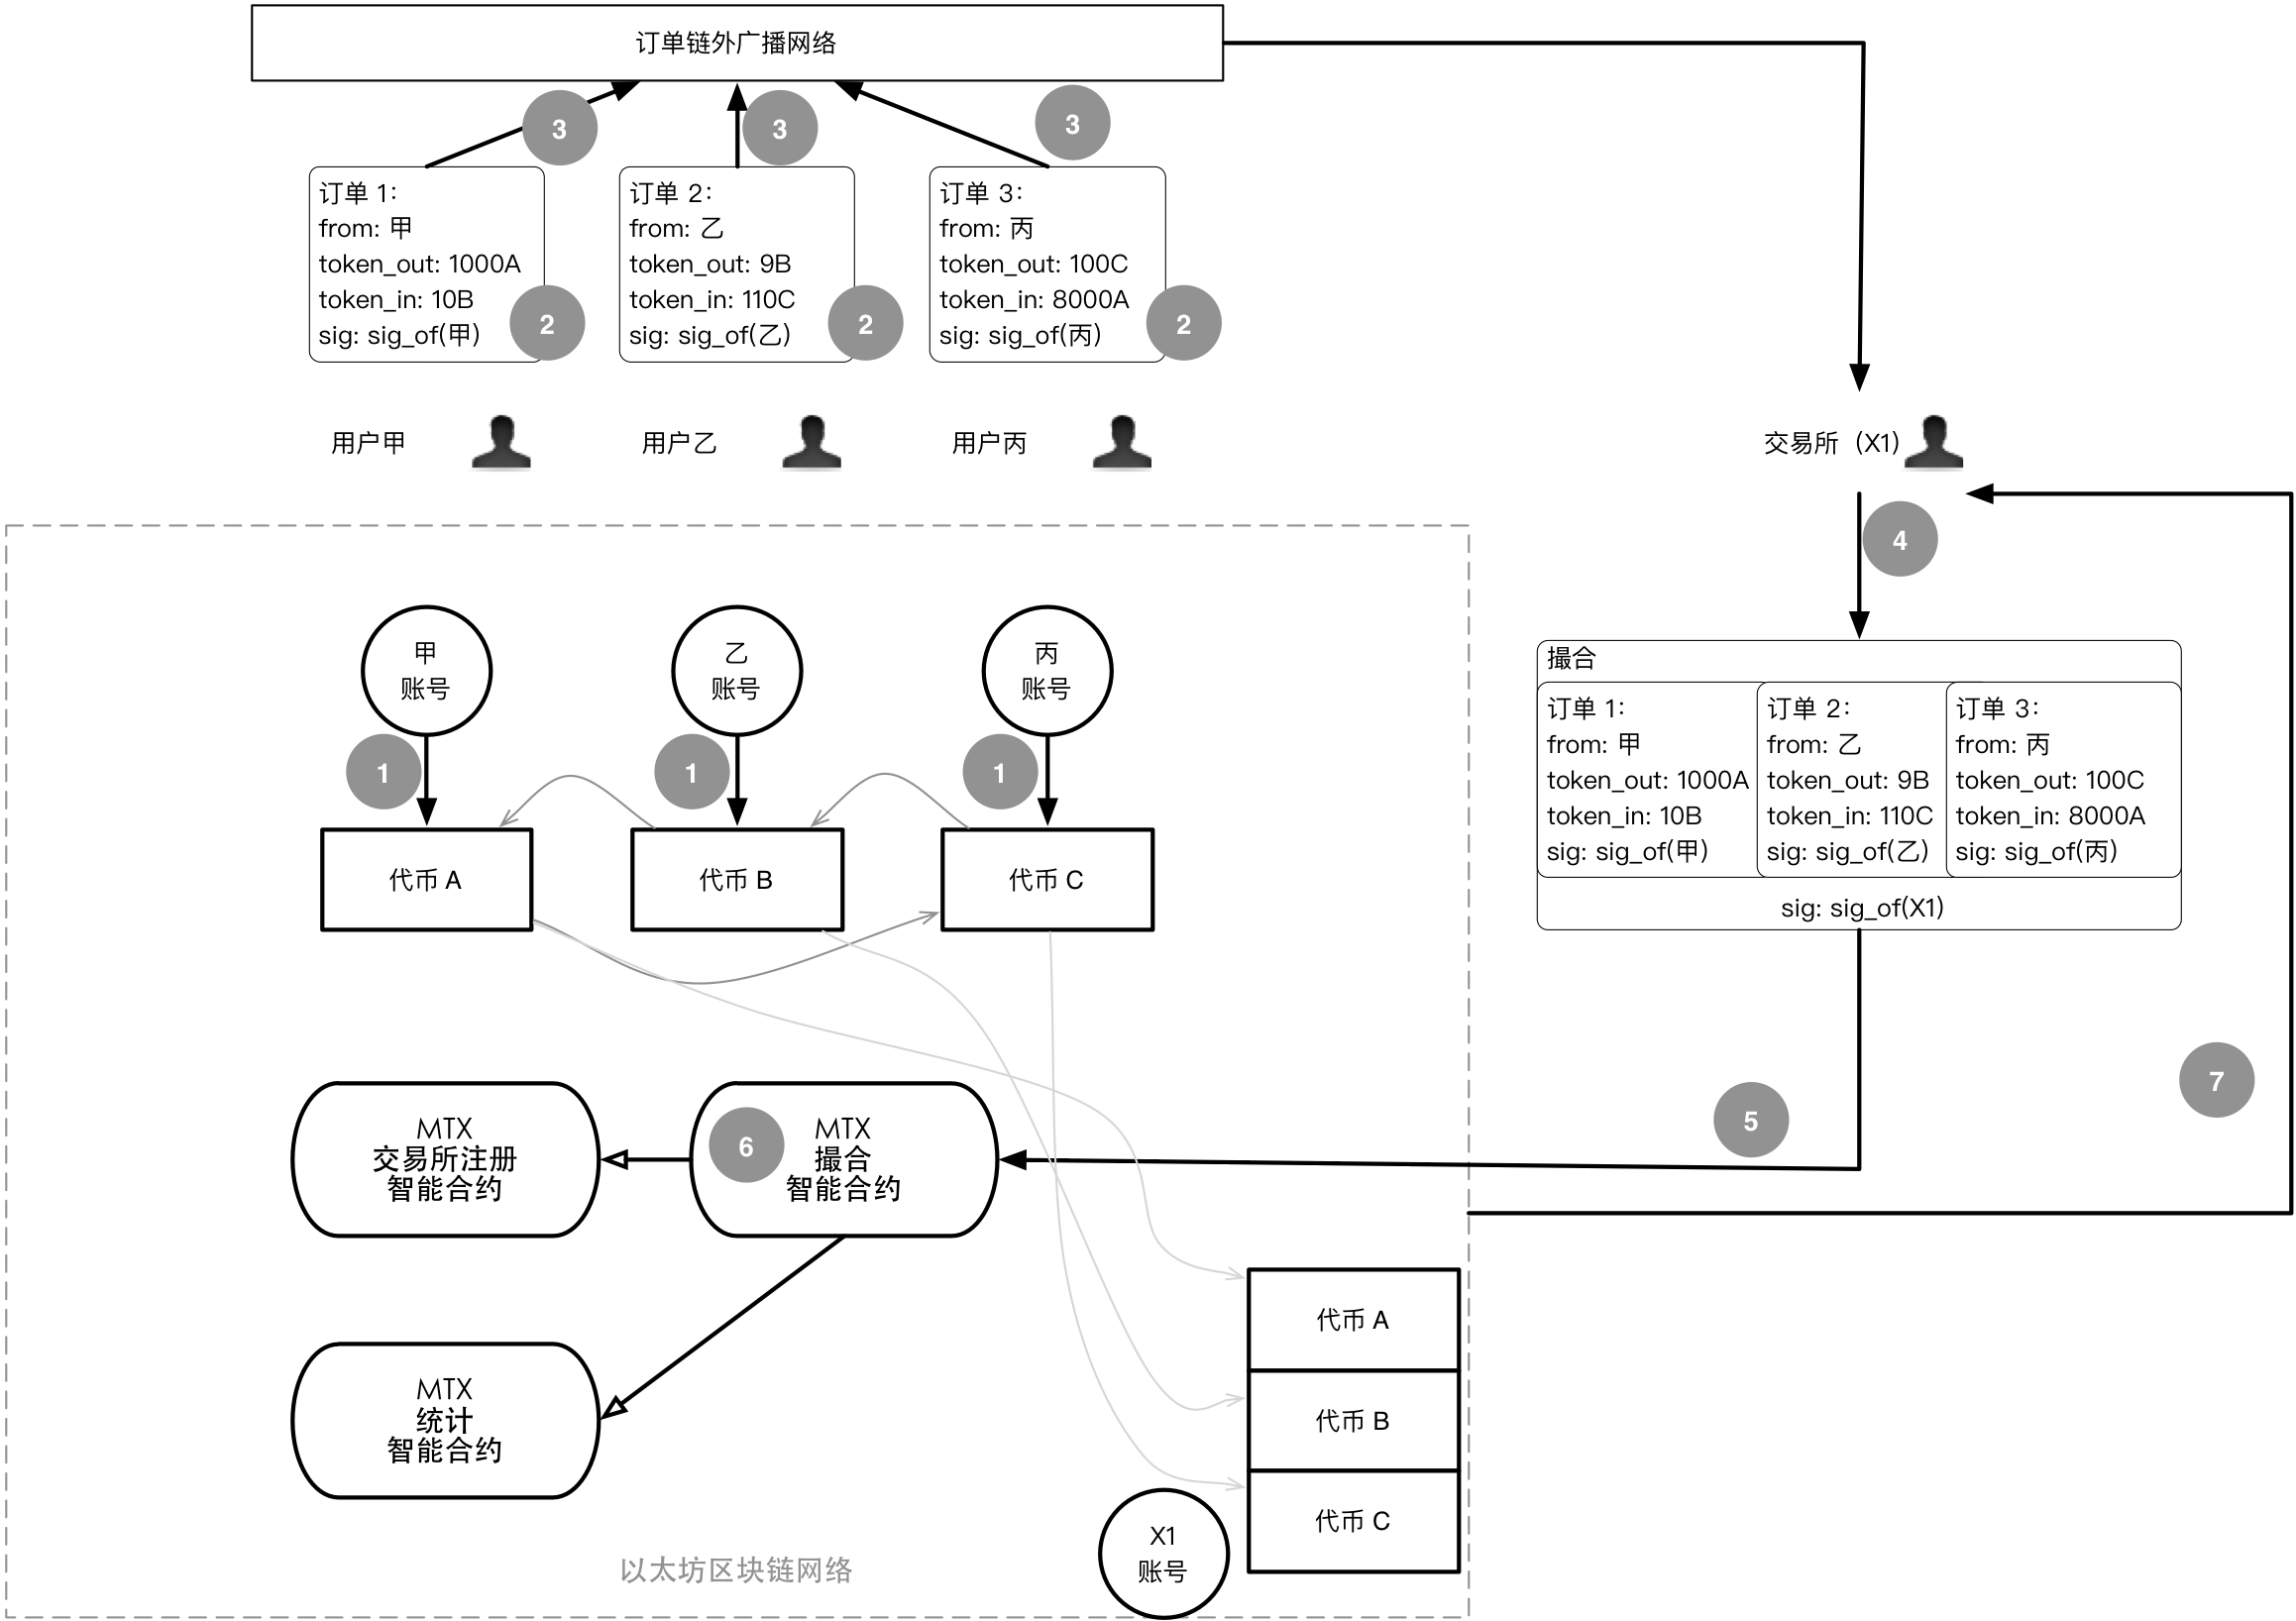
\includegraphics[height=10cm]{images/protocol.png}
\caption{MTTP:Figure shows mix and match 3 orders}
\label{fig: MTTPprotocol}
\end{figurehere}
\end{center}

Figure 1 presents the general sequence of steps used for three parties transaction under MTTP:

\begin{enumerate}
 \item User A,  B and C authorize MTTP matching smart contract to manipulate their account for token trading and exchanging. From figure,  Contract will transfer out 1000 token A from User A’s account,  and transfer out 9 token B from User B’s account,  100 token C from User C’s account;
 \item User A,  B and C place their own orders with signature on their private keys. Thus,  all the orders go into a medium and ready to exchange - Order A is selling no more than 100 token A and purchase no less than 10 token B; if the order is partially matched,  then exchange rate between A to B should be no less than 1000/10=100.00 (Selling tokens divided by purchasing tokens). We will illustrate other involved parameters in chapter 3.7;
 \item User A,  B and C continue to send their order one of multiple exchanges;
 \item After the exchange received three separate orders,  they will replace them into corresponding orderbook, while update new block and calculate each order’s status in order to match the set order - since we call it circulation exchange or matching exchange. Once all the orders are confirmed and successfully mix-matched;
 \item Exchange will send out a signature to MTTP matched smart contract address;
 \item Matching smart contract to verify quadruple signatures in order to verify three orders’ closing. If closing is failed,  then terminate the conract(exchange still cost certain gas); vice verse,  smart contract needs to calculate the proceed and cost for each users, then complete the token exchange. During the each steps, matching smart contract will use MTTP Registration Contract to calculate all the fees and discount; discount; before closing,  system will also need to use MTTP Stats Contract to update database.
 \item Exchange starts receiving new block and new data from the chain in order to upgrade the orderbook then to mix-match the orders.
\end{enumerate}


\subsection{Definition of Symbol}

First we would introduce the definition of each symbol.
\[
\begin{split}
&C_{i}\text{: \ }\text{$i$ is set of token.}\\
&O_{i\rightarrow j}\text{: \ }\text{stands for selling a token, $C_{j}$stands for purchasing a token.}\\
&s_{i\rightarrow j}\text{: \ }\text{number of token sold $C_{i}$.}\\
&b_{i\rightarrow j}\text{: \ }\text{number of token purchased $C_{j}$.}\\
&r_{i\rightarrow j}\text{: \ }\text{exchange rate,  $s_{i\rightarrow j} / b_{i\rightarrow j}$.}
\end{split}
\]


We underlined the symbols to emphasis on their original numbers. For example $\overline{s}_{i\rightarrow j}$ and $\overline{b}_{i\rightarrow j}$ stands for number of token from the original order

\subsection{Fixed order exchange rate\label{sec: consistrate}}

For instance,  if the order is fully completed, $s_{i\rightarrow j} = 0$. Otherwise numbers will be showed as:
$s_{i\rightarrow j} / b_{i\rightarrow j} = \overline{s}_{i\rightarrow j}/ \overline{b}_{i\rightarrow j}$,
after MTTP updated: $r_{i\rightarrow j} = \overline{r}_{i\rightarrow j}$.


\subsection{Agreement\label{sec: reducability}}


We can use token $C_j$ to connect two orders ( $O_{i\rightarrow j}$ and $O_{j\rightarrow k}$ ),  regard as a order for selling token $Ci$,  other is purchasing order $C_k$. we use $O_{i\rightarrow j\rightarrow k}$ to display this order. Thus mix and match with order $O_{i\rightarrow k}$:

\begin{equation}
s_{i\rightarrow j\rightarrow k}=min(b_{i\rightarrow j}, s_{j\rightarrow k}) \cdot r_{i\rightarrow j}
\end{equation}

\begin{equation}
b_{i\rightarrow j\rightarrow k}=min(b_{i\rightarrow j}, s_{j\rightarrow k}) / r_{j\rightarrow k}
\end{equation}

\begin{equation}
r_{i\rightarrow j\rightarrow k}= r_{i\rightarrow j}\cdot r_{j\rightarrow k}
\end{equation}


We will introduce a concept of ordering-chain. It contains two or more orders. Both two orders exchange same type of token except the last order. Additionally,  final order’s purchasing token should be differ from initial order’s selling token (it will become a circulation if its same type of token).

\[ s_{0\rightarrow ...\rightarrow n} =
 \begin{cases}
  s_{0\rightarrow 1}   & \quad \text{as } n \text{ = 1}\\
  min(b_{0\rightarrow ...\rightarrow n-1}, s_{n-1\rightarrow n}) \cdot r_{0\rightarrow ...\rightarrow n-1} & \quad \text{as\ } n \text{ $>$ 1}\\
 \end{cases}
\]

\[ b_{0\rightarrow ...\rightarrow n} =
 \begin{cases}
  b_{0\rightarrow 1}   & \quad \text{as } n \text{ = 1}\\
  min(b_{0\rightarrow ...\rightarrow n-1}, s_{n-1\rightarrow n}) / r_{n-1\rightarrow n} & \quad \text{as\ } n \text{ $>$ 1}\\
 \end{cases}
\]


\[ r_{0\rightarrow ...\rightarrow n} = \prod_{i=0}^{n-1}{r_{i\rightarrow i+1}}
\]


\subsection{Mix and Match Trading}

Centralized exchange happens between two kinds of tokens/currencies; However,  MTTP exchange involves multiple tokens/currencies through connecting each orders to complete the exchange.


\begin{definition}[Circular Trading] Let $C_{0}$, $C_{1}$, $\cdots$, $C_{n-1}$ be $n$ different kinds of token, $O_{0\rightarrow 1}$, $\cdots$, $O_{i\rightarrow i\oplus 1}$, $\cdots$, $O_{n-1 \rightarrow 0}$ be $n$ orders. Those orders can mix and match with different kind of tokens for trading:
$$O_{0\rightarrow 1} \rightarrow \cdots \rightarrow O_{i\rightarrow i\oplus 1} \rightarrow \cdots \rightarrow O_{n-1\rightarrow 0} \text{, }$$
where $n$ is the length of the circulation, and $i\oplus 1 \equiv i+1 \mod n$.
\end{definition}

Once the prices match the orders under circumstance,  we could start to complete trading in this circle.

\subsubsection{Price\label{sec: matchprice}}
We will introduce an example for a better understanding of price mechanism. Assume three kinds of token are $C_{0}$, $C_{1}$ and $C_{2}$, three separate orders:$O_{0\rightarrow 1}$, $O_{1 \rightarrow 2}$ and $O_{2 \rightarrow 0}$. Easy to approve, as if $r_{0 \rightarrow 1} \cdot r_{1 \rightarrow 2}\cdot r_{2 \rightarrow 0} = 1$, when three orders could complete the exchange. As $r_{O \rightarrow 1} \cdot r_{1 \rightarrow 2}\cdot r_{2 \rightarrow 0} > 1$. We named the first situation as \texttt{original matching}, Second as \texttt{discount matching}.

According to MTTP protocol, each order in the circulation would share the same price. For instance, if discount rate is $\gamma$, then price for each order will be:
$r_{0\rightarrow 1} \cdot (1-\gamma)$, $r_{1\rightarrow 2} \cdot (1-\gamma)$, $r_{2 \rightarrow 0} \cdot (1-\gamma)$, and satisfied:
\begin{equation}
r_{0\rightarrow 1} \cdot (1-\gamma)\cdot r_{1\rightarrow 2} \cdot (1-\gamma) \cdot r_{2 \rightarrow 0} \cdot (1-\gamma) = 1
\end{equation}
We can find out:
\begin{equation*}
\gamma = 1- \frac{1}{\sqrt[3]{r_{0\rightarrow 1} \cdot r_{1\rightarrow 2} \cdot r_{2\rightarrow 0}}}\text{.}
\end{equation*}
In the other circumstance, if transaction cross $n$ orders, \texttt{discount rate}:
\begin{equation*}
\gamma = 1- \frac{1}{\sqrt[n]{\prod_{i=0}^{n-1} r^i}} \text{,}
\end{equation*}
where $r^i$ is the order turnover rate of $i$-th order.Obviously, only when the discount rate is $\gamma \ge 0$, transaction can be completed; and $i$ order's $O^i$ actual exchange rate $\hat{r^i} = r^i \cdot (1-\gamma)$, $\hat{r^i}\le r^i$.

%在章节\ref{sec: fee}中, 我们还会详细介绍交易所通过MTTP代币抵押的原因和细节, 最终的结果是每个交易都被迫给自己的撮合的实际兑换率打个折扣, 即\texttt{交易所折扣}.假交易所$X$的交易所折扣为$\mu$, 那么由该交易所撮合是, 最后的实际成交兑换率为:$\hat{r^i} = r^i \cdot (1-\gamma) \cdot (1-\mu)$


\subsubsection{Volume\label{sec: matchquantity}}

To find out the lowest value order can help to figure out the total volume. For instance, $i$ is the lowest value order, then number of token sold from each order $\hat{s}$ and number of token brought $\hat{b}$ from each order can be find:

\[
\begin{split}
&\hat{s}^{i}=\overline{s}_i\text{, } \hat{b}^{i}=\hat{s}^{i}/ \hat{r}^i\text{, }\text{;}\\
&\hat{s}^{i\oplus 1}=\hat{b}^i\text{, } \hat{b}^{i\oplus 1}=\hat{s}^{i\oplus 1}/ \hat{r}^{i\oplus 1}\text{;}\\
&\hat{s}^{i\oplus 2}=\hat{b}^{i\oplus 2}\text{, } \hat{b}^{i\oplus 2}=\hat{s}^{i\oplus 2}/ \hat{r}^{i\oplus 2}\text{;}\\
& ...
%\text{.}
\end{split}
\]
where $\overline{s}_i$ is the the balance left after order partially traded.

\subsubsection{Cost and Fee\label{sec: fee}}

Exchanges normally charge transaction fee. For instance,  we assume fee will be calculated in MTTP token $MTC$, order ID is $i$ and total fee for completing the transaction is $m^i$:

\begin{equation*}
f^i = b^i \cdot m^i / \overline{b^i}
\end{equation*}


In order to encourage exchange to offer best rate for the users,  MTTP would distribute profit from \texttt{cost saving} to the exchange. as an order $O^i$,  if price for purchasing is $b^i$( $b^i \le \overline{b^i}$ ),  then we define the from saving cost:

\begin{equation*}
\Delta^i = b^i \cdot r^i \cdot \gamma
\end{equation*}

If MTTP requires every order to set up a saving cost distributing rate $\theta^i$, and minimum distributing ratio is $\Theta$. Then order $O^i$ should pay to exchange:


\begin{equation*}
f^i = \Delta^i \cdot \Theta = b^i \cdot r^i \cdot \gamma \cdot \Theta
\end{equation*}

Since the income from cost saving among each matching trade:

\begin{equation*}
F = \sum^{n-1}_{i=0} b^i \cdot r^i \cdot \gamma \cdot \Theta
\end{equation*}

In order to encourage $MTC$ usage,  if the order has no preset token fee $m^i$, or $m^i=0$, then the actual ratio is 100\%,  regardless of the relevant hash in this order. As if none of the order has set up this rate $\Theta=100\%$,  then all proceeds from the saving will go into exchange.

In next chapter,  we will introduce a token pledge policy,  smart contract will list out each exchanges depositing tokens and rank them up. Secondly calculate a \texttt{mandatory discount cost} for each exchange, $\lambda$, this figure will affect the total cost. Meanwhile, exchange can also offer some discount, $\eta$. Total cost for completion a full trading:

\begin{equation*}
F =(1-\lambda)\cdot (1-\eta) \cdot \sum^{n-1}_{i=0} (b^i \cdot r^i \cdot \gamma \cdot \Theta + b^i \cdot m^i / \overline{b^i})
\end{equation*}


\subsubsection{Discount}
MTTP requires exchange platform offering discount for each transaction,  discount fee depends on the number of deposit token $MTC$. The higher the rank,  the lower fee will charge; For example Rank $n$'s cost will be:

$$\lambda_{n} = 0.05\cdot(\ln (n+e-1) - 1)\text{.}$$
Details below:


\begin{table}[hbt]
 \centering
\begin{tabular}{p{3.5cm}|p{3cm}} %设置了每一列的宽度, 强制转换.
Deposit Ranking $n$ & cost for discount $\lambda$ \\ %用&来分隔单元格的内容 \\表示进入下一行
  \hline
1 & 0\%\\
\hline
2 & $1.57\%$\\
\hline
10 & $7.31\%$\\
\hline
20 & $10.39\%$\\
\hline
99 &$18.06\%$\\
\hline
100 &$18.11\%$\\
\hline
1000 &$29.55\%$\\
\hline
1001 &$30.00\%^*$\\
 \end{tabular}
\caption{Deposit $MTC$ Ranking and cost for discount} %显示表格的标题
\end{table}


For those exchanges ranked under 1001 and those undeposited exchanges, 30\% cost will apply.

Figure \ref{fig:discount} shows, $\lambda_{2} - \lambda_{1} \gg \lambda_{100} - \lambda_{99}$.

\begin{center}
\begin{figurehere}
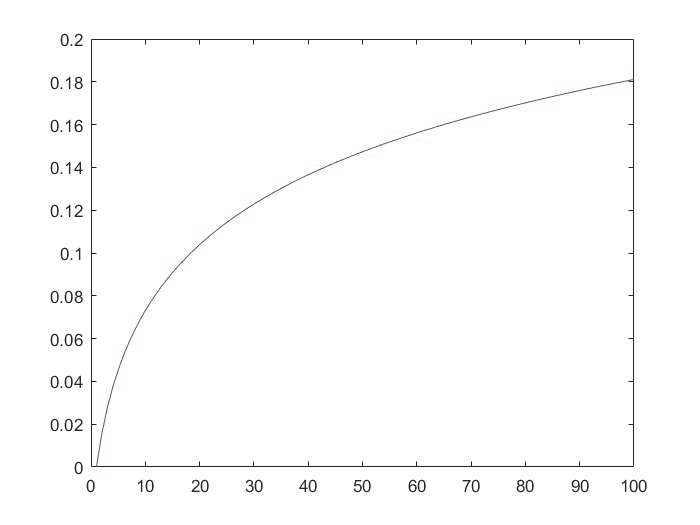
\includegraphics[height=8cm]{images/exchange-discount.png}

\caption{$MTC$ token deposit rank and cost for discount}
\label{fig:discount}

\end{figurehere}
\end{center}


\subsection{Fraud and Attach Protection}

\subsubsection{Exchange Covered Interest Arbitrage}

MTTP is trying create a fair ecosystem and find a balance between customers and exchanges. Firstly,  we will explain how exchange could archive a zero risk covered interest arbitrage.

Assume there are two orders $O_{a\rightarrow b}$, $O_{b\rightarrow a}$, form a loop, $r_{a\rightarrow b} \cdot r_{b\rightarrow a} > 1$. Exchange can input three new orders between those two. $O_{b\rightarrow c}$, $O_{c\rightarrow d}$, $O_{d\rightarrow b}$, to create a five orders-loop,  $r_{a\rightarrow b} \cdot r_{b\rightarrow c} \cdot r_{c\rightarrow d}\cdot r_{d\rightarrow b}\cdot r_{b\rightarrow a} = 1$. Exchange could make all the possible cost down to zero, once the transaction completed, it's like zero risk covered interest arbitrage
and $O_{b\rightarrow c}\rightarrow O_{c\rightarrow d}\rightarrow O_{d\rightarrow b}$. In order to stop those matter, MTTP requires:{\bfseries verified loop must not be able to create more sub-loop to trade}.

\subsubsection{Rejection Service}

MTTP allows exchange to select the order. Order can be sort by token,  quantity,  number and others. Condition can be modified,  hidden or public.

\subsubsection{Mass Small Order}
User can send out mass small orders to attach the exchange. Due to tiny profit from those orders,  exchange would reject most of them.

Few exchanges can use same method to attack other exchanges. However this would not work in MTTP ecosystem.

\subsubsection{Insufficient Balance}

Multiple order can be sent out at one time,  while the account balance is actual zero. Thus,  even those orders been sent to exchange. Exchange would detect the zero balance account and pause the transaction. This action could increase large time cost. In conclusion,  set up regulation to block those suspicious account in the future.

\subsubsection{Trade Matching Filch}

A dodgy exchange could monitor those unclosed deal from the internet. In order to protect us from cyber-fraud. We require exchanges to complete two steps in order to submit the order:
\begin{itemize}
  \item A transaction has saved on blockchain,  and update the record,
  \item Data has been recorded on blockchain,  exchange provide detailed info.
\end{itemize}
Hash rate:
$$h = H(r,  nonce)\text{, }$$
where $H()$ is a one-way hash function, $r$ is order record. Hash Hash function contains a random number $nonce$.

\subsection{Market Insights\label{sec: marketdepth}}

Exchange no need to offer market depth data. Under this ecosystem,  both single organization and corporation can possibly pool all the un-closed orders into one market depth data. We can find out trading data between any two ERC20 tokens according to the argreement in chapter 3.3.

\subsection{Database Formula\label{sec: dataformat}}

All the orders can be illustrated into one module due to adopting OTC module. This module contains both digital signature and all parameters. Before the signature,  connect the parameter data from the orders into a set data,  calculate the order’s hash by using Keccak SHA3 methodolgy,  then sign on this account’s private keys with ECDSA.


\begin{verbatim}
message Order {
 address protocol;
 address owner;
 address outToken;
 address inToken;
 uint256 outAmount;
 uint256 inAmount;
 unit256 expiration
 unit256 fee;
 uint8 savingShare;
 bytes signature;
}
\end{verbatim}

Though there’s no indicated price from the order,  but we are still able to find out through the formula: $outAmount / inAmount$ to get exchange rate r. All the actual exchange rate must be less than $r$. A user-friendly exchange should allow user to input $outAmount$, $inAmount$,  selling and asking price and use any two of those numers in order to calculate the missing $outAmount$ 或 $outAmount$ figure.

Actual orders can be defined in two different ways: Definition A - transaction can be completed once number of token sold reaches $outAmount$ ; Definition B - transaction can be completed once number of token purchased reaches $inAmount$; Therefore,  we can setup a quote for exchange and mix-matching contract to help to define the trade. At our initial version,  we would pre-set Definition A method.

Exchange could create a circular trading from below date:
\begin{verbatim}
message Match {
  Order[] orders;
  address fee Recipient;
  unit256 additional Discount; // eta
  bytes signature;
}
\end{verbatim}


\subsection{Order Status\label{sec: orderstate}}


Order cannot be modified since it’s been signed and announced. Data will be updated on the blockchain once smart contract find the matched order. Thus $inAmount$ and $outAmount$ will modified in corresponding with updated price. If $inAmount / outAmount$ shows 0,  it means the order has been fully closed. For example,  if the user wants to cancel the order,  a special request will be filed,  $inAmount / outAmount$ will be 0 to close the order. An expired order will not be updated on the blockchain - it can be tracked through the final cutting time. Hence,  we expect most of the orders will be expired or invalided.

\subsection{Smart Contract\label{sec: contracts}}

MTTP consists of many smart contracts,  including:

\begin{itemize}
 \item \textbf{Mix-Matched Contract}is responsible for ensuring each order status in the loop,  calculating the price and volume,  transferring and interaction with other smart contracts,  API for MTTP;
 \item  \textbf{Order Contract}update order database and support cancelling policy;
 \item \textbf{Registration Contract}maintain and upgrade service for exchanges who accepted MTTP,  support the token deposit from exchange and defaulted parameters backup;
 \item \textbf{Stats Contact}calculate the exchange volume and price between two tokens.

\end{itemize}

\begin{comment}
\subsection{支持ENS\label{sec: registration}}

\end{comment}

\section{Token $MTC$ \label{sec: protocoltoken}}


We will issue a token base on ERC20 Ethereum Token Standard called $MTC$(display in italics).


\subsection{Token Application}

$MTC$ will be use in below areas

\begin{itemize}
 \item \textbf{Gas Fees} --- $MTC$ can be used for transaction fee for exchange. It will be easy and productive for the exchange to calculate all the cost in $MTC$. Same as request sender and receiver. We have mention this from previous chapter\ref{sec: fee}.
 \item \textbf{Deposit for Exchange Registration} ---Decentralized exchange mechanism has no limits on location or time. Thus,  those high turnover exchange would receive more orders and get more users. Hence,  we have setup a policy for those exchange that allow them to use $MTC$ to deposit into smart contract in order to increase exchange's credibility. Moreover,  it can also protect user from certain circumstance.
\end{itemize}

\subsection{Decentralization Mechanism}
Regulation has been updated as well as exchange's mechanism. Any $MTC$ holders have the voting power $S$, and number of the pledging $N$ and pledging time $CoinAge$
$$S = f(N,  CoinAge)\text{, }$$
where $CoinAge = H_{c}-H_{s}$. Joining CoinAge is to protect customers from speculations.

Decentralized mechanism include token registration, exchange registration, stat hash, deposit scale, maximum length, discount hash, subcontract address.
 \begin{itemize}
   \item \textbf{token registration} MTTP would adjust token,  low trading volume will be eliminated and new popular token will be replaced. however all the adjustment have to be recorded on smart contract.
  \item \textbf{exchange registration} Only those exchanges accept MTTP would allow to start trading.
   \item \textbf{stat hash} Data will increase to certain amount after a long period operating. The more data exchanges have,  the more accurate system computation ability has.
  \item \textbf{deposit scale} Deposit for each exchange should be scalable. if the amount is huge,  the liquidation gets worse; verse vice.
   \item \textbf{maximum length} Technically, more orders can create more profit,  however the risk of failure also increase. As well as the trading cost.
   \item \textbf{discount hash} Discount hash will be adjust with the market. Below figure shows, blue line represents normal market, yellow line represents supply market, red line represents demand market.
\begin{center}
\begin{figurehere}
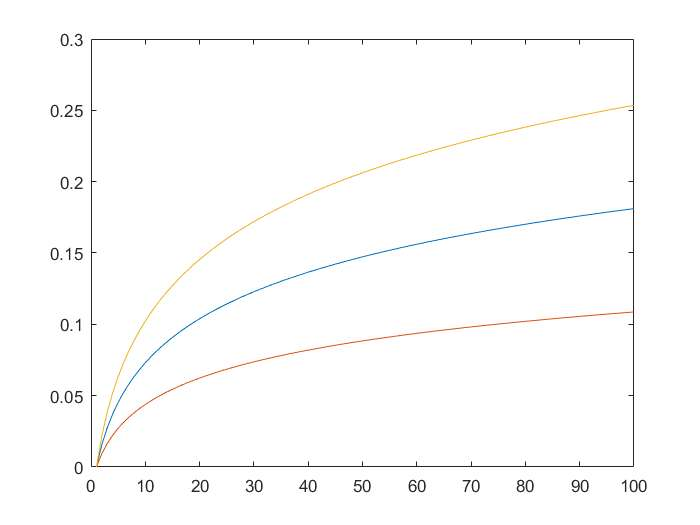
\includegraphics[height=10cm]{images/rate_adjust.jpg}
\caption{discount rate after adjustment}
\label{fig: dischargeRateAdjust}
\end{figurehere}
\end{center}

   \item \textbf{subcontract address} If MTTP exchange based on Ethereum ecosystem,  then smart contract cannot be modified. Therefore,  update MTTP's subcontract in order to modify subcontract address.
 \end{itemize}

%\footnotemark

\subsection{Token’s Liquidation}

MTTP’s token is based on ERC20 Ethereum Token Standard and it can be liquidated through MTTP smart contract. It means MTC trading can be made out of centralized exchange. All the ERC20 Ethereum tokens can be exchanged to MTC token( assume pre-order is MTC,  with zero fee) by adopting MTTP’s decentralized mechanism.


\section{Exchange\label{sec: exchange}}

Exchange is unable to guarantee all the transaction could make profit after adopted MTTP. First reason is high operating cost. Secondly,  high expectation cannot match the actual outcome. There are few other reasons would cause this sutuation. Overall,  both exchange platform and other parties have reciprocal relationship: exchange looks for profitable order; while order senders look for exchange with lowest fee.
Exchange is not responsible for users ERC20 token after accepting MTTP. The workload has move from money despit,  withdraw,  internal virtual account management to mix-matched order service. Meanwhile,  for the users,  MTTP does not require customer to deposit or lock any asset, that means asset have zero risk to get stolen, at same time single order can mix and match multiple trades.
For Non ERC20 asset,  exchange can offer asset tokenization service.

\subsection{Comparing Regular and MTTP Exchange}
In a regular exchange,  “Maker” send a order and “Taker” receive order. The exchange price highly depends on sender’s end. Under MTTP circumstance,  it has adopted Over-The-Counter (OTC) module.
In current market,  there is considerably high risk for users to trade in those platform,  no law to regulate the exchange if they vanish. But with MTTP,  users do not to deposit money to the exchange anymore. All the transactions will be made among users coin address.
Another feature for MTTP is that it has change the “Trading Pair”concept. Transaction can be completed with multiple paries instead of 2 parties in current exchange.


\begin{table}[hbt]
 \centering
\begin{tabular}{p{5cm}|p{3.5cm}|p{3cm}} %设置了每一列的宽度, 强制转换.
&Centralized Exchange & MTTP Exchange \\ %用&来分隔单元格的内容 \\表示进入下一行
  \hline
Deposit for the order& Yes & No \tablefootnote{MTTP交易所无需托管下单资金 --- 交易用代币存放到自己区块链地址中, 成交前无需要转账.资产丢失或者被盗风险为零.} \\
\hline
Frozen Account& Yes & No \tablefootnote{MTTP交易所无需冻结下单资金 --- 用户下单后依然可以任意动用账户任何资金, 将资金部分或全部转移走等同于部分或全部撤单.} \\
\hline
Deposit/Withdraw& Yes & No \tablefootnote{MTTP允许用户的同一个订单被多家MTTP交易所同时撮合, 并可以被多家交易所不同程度部分或全部成交.}\\
\hline

Internal Trading Risk& Yes & No\tablefootnote{MTTP交易所撮合全部基于区块链智能合约, 数据不可更改, 完全开放透明.}\\
\hline
Customer loss from exchange closing& Yes & No\tablefootnote{MTTP交易所如果不提供代币发行职责, 交易所倒闭对用户没有任何影响 --- 好比矿工倒闭对区块链账户也没有影响一样.交易所只负责撮合, 清算转账通过智能合约完成.所有资产一直在区块链用户自己的账户里.}\\
\hline
Transaction is the main income& Yes & No\tablefootnote{MTTP交易所的交易手续费为辅助收入, 主要收入为成交的“成本节约分润”, 这样会激励撮合价格最优订单.}\\
\hline
Accept Legal Currency& Yes & Yes\tablefootnote{MTTP交易所对法币的支持是通过资产代币化, 需要将法币在区块链上做ERC20代币发行.}\\
\hline
Can be traded among multiple exchanges& No & Yes \tablefootnote{MTTP允许用户的同一个订单被多家MTTP交易所同时撮合, 并可以被多家交易所不同程度部分或全部成交.}\\
\hline
Fairness for Maker and Taker& No & Yes \tablefootnote{MTTP协议要求成交接近中间价, 而不是过度倾向于Maker的价格.}\\
\hline
Mix and Match Trading& No & Yes\tablefootnote{MTTP交易所支持环路发现, 能最大程度找到最好的匹配订单.}\\
\hline
Supervision & Strong & Weak\tablefootnote{MTTP交易所不保存资金, 清结算通过开源智能合约完成.因此如果不提供资产和跨链代币发行服务, 监管的必要性很弱.}\\

 \end{tabular}

\caption{Contrast between centralized exchange and MTTP exchange} %显示表格的标题
\end{table}

%\footnotemark

\section{Summary\label{sec: summary}}

We describe a protocol that facilitates decentrazlized exchange of ERC20 tokens on the Ethereum blockchain. MTTP allows multi token transaction exchnage,  as well as it accepts exchange liquidation on blockchain; This whitepaper has explained how the mechanism work under different circumstance. In additional,  the benefit that MTTP has brought to current exchange mechanism.
MTTP protocol fits any ERC20 and smart contract blockchain platform. After many discussion,  our team will develop MTTP on the Ethereum blockchain.
We also plan to create a non profit foundation for MTTP through crawdsale and issue ICO.

\section{Acknowledgements\label{sec: acknowledgement}}

We would like to express our gratitude to our mentors,  advisors and to the many people in the community that have been so welcoming and generous with their knowledge. In particular,  we would like to thank Xing,  Jiang; Xiaochuan Wu; Zhen, Wang and Jun, Ma for reviewing and providing feedback on this work. We are also welcoming more feedbacks from community.

\newpage
\bibliography{whitepaper}
\bibliographystyle{unsrt}

%\newpage
%
%\begin{appendices}
%\section{$MTC$ Token Crowdsale\label{sec: ico}}
%
%We plan to issue 100 million MTC token,  8000 million tokens will be allocated to crowdsale participators. and rest 20 million tokens will be allocated to the foundation initiator for maintain and developing the community in the next 5 years.
%
%ICO will start pre-sale to investors and crowdsale in 2017 July. We plan to raise XXXX ETH
%Initial spending plan;
%
%\begin{table}[hbt]
% \centering
% \begin{tabular}{l|c}
%   Purpose    & Percetage\\
%  \hline
% Tech Development  & 50\% \\
% Community Building & 20\% \\
% Marketing     & 15\% \\
% Legal and Law   & 15\% \\
% \end{tabular}
% \caption{ Plan for token expense}
%\end{table}
%
%
%
%Project ICO and Timetable
%\begin{table}[hbt]
% \centering
% \begin{tabular}{l|l}
%Time  & Target\\
%  \hline
% 2017/06 & Whitepaper release, Project start-off \\
% 2017/07 & Module Development Completion \\
% 2017/08 & MTTP open source commitee(Foundation)set and Pre ICO closed \\
% 2017/08 & ICO Schedule \\
% 2017/09 & ICO start \\
% 2017/10 & ICO close and release result \\
% 2017/11 & $MTC$Token IOU launch at exchange \\
% 2017/12 & Test $MTC$ token on ETH \\
% 2018/02 & Commencement \\
% 2018/04 & Issue $MTC$ token on ETC \\
% \end{tabular}
% \caption{Project Schedule}
%\end{table}
%
%\subsection{ETH/ETC Due-chain issue\label{sec: chains}}
%
%Though we only accept ETH as our ICO token,  but we also consider ETC token's potential on developing smart contract. Hence,  we will issue our token $MTC$ on both Ethereum (ETH)and Ethereum Classic(ETC).
%
%
%\subsection{Risk Awareness\label{sec: risks}}
%
%Initial crypto-token offering (ICO) now is a popular way for crowdsale,  it contains certain risks. Participators should be fully aware of all the potential risk and The MTTP Foundation hereby expressly disclaims its liability,  and shall in no case be liable to any person,  for:
%\begin{itemize}
% \item any person’s participation in the Campaign in violation of any anti-money laundering,  counter-terrorism financing or other regulatory requirements that are imposed in any jurisdiction;
% \item any person’s participation in the Campaign in violation of any representation, warranty,  obligation,  covenant or other provision under this Prospectus,  and the resulting failure or inability to retrieve his/her payment or to claim relevant purchased $MTC$ for Crowdsale;
% \item early termination of the Campaign for any reason;
% \item failure or abortion of the Quantum development and resulting failure to deliver the purchased $MTC$ for Crowdsale to the Purchasers;
% \item any risk factors disclosed in this Prospectus and any damage,  loss, claim, liability, punishment, cost or other adverse impact that is caused by, associated with, in connection with, incidental to or consequential to that risk factor.
% \item if there is any separate agreement between a Purchaser and a Crowdsale Intermediary,  this Prospectus shall take precedence over that agreement in all respects. The MTTP Foundation shall in no case be bound by,  and hereby disclaims any liability under,  the foregoing agreement.;
% \item failure or abortion of the MTTP development and resulting failure to deliver the purchased $MTC$ for crowdsale to the Purchasers;
%
%\end{itemize}
%
%
%
%\end{appendices}
\end{document}
